\chapter{Statistical Machine Translation}
Even though there are many ways that translation from one language to another can be done\cite[p. 5-6]{trujillo2012translation}, many machine translation (MT) scholars now consider statistical machine translation (SMT) as the most effective way for developing efficient large-scale translation systems\cite[p. xi]{koehn2009statistical}. The main idea behind SMT is to use large text translations from one language to another (parallel corpora) to generate translation tables, and then use good-quality content (monolingual corpus) of the target language to train its model, that is teaching the system about the general structure of that particular language so that is the system is able to evaluate generated translations and pick the most likely among them by using set statistical parameters.

To produce a good translation model, you need to have a large dataset of parallel corpora of high quality to use when developing translation rules for your model. According to Franz Josef Och, an SMT pioneer who created started the Google Translate project, you need at least a parallel corpora of 50-200 million words\cite{och2005statistical}.  You also need to have a very large monolingual corpus, more than a billion words according to Och, to use when training the target language model\cite{och2005statistical}. In addition to this you have to \textit{tune} the translation model. \textit{Tuning} is the process in which the translation performance of the model is optimized by using a different parallel corpus that is of greater or equal quality than the one that that was used in the training stage. Given these two, and other, steps involved in developing an SMT system heavily employ statistical machine learning techniques, it is only reasonable that I discuss the basics of statistical machine learning before diving into the specifics of SMT systems. 

\section{Statistical Machine Learning}

After the development of digital computers during the last half of the $20^{th}$ century, there have been multiple attempts of using machines to perform several tasks such as speech recognition, text translation, and data analysis. The process of teaching a machine the basics how to perform a certain task, and then letting the machine learn the rest on its own, is called ``machine learning''\cite{princetonml}.

Statistical machine learning is a branch of machine learning that uses data to generate statistical models that can then be used as functions when modeling new data inputs. To develop an SMT system, one uses large amounts of corresponding texts from both the source language and the target language as inputs of a learning algorithm that then generates statistics of equivalence between the two bodies of texts in form of probabilities. These probabilities are then used as inputs of another program that does the actual translation. 

The resulting translating system can take a string of text in the source language and uses the rules, in this case statistical probabilities generated by the first algorithm, to output the best possible translation according to its rules. This is a very simplified example as it doesn't include all the steps involved in training an SMT model using prominent SMT systems such as Moses\cite{koehn2007moses}, but it provides enough details to showcase how basic concepts from machine learning are applied and used by SMT systems and SMT-based translation models. 
\section{The Mathematics of Machine Translation}
%%%%%%%%%%%%%%%%%%%%%%%%%%%%%%%%%%%%%%%%%%%%%%%%%%%%%%%%%%
In this section, I explore the Mathematics behind some of the main SMT concepts as discussed in an article by Brown \etal entitled \textit{``The Mathematics of Statistical Machine Translation: Parameter Estimation''}\cite{brown1993mathematics}.
\subsection{Probabilities in Translation}
Suppose we are given an English sentence $e$, and we are trying to translate it to its corresponding Kinyarwanda sentence $k$, $P(k|e)$ is the probability that we will get the Kinyarwanda translation $k$ when starting with the English sentence $e$. $P(k)$ is the prior probability that $k$ happens based on our system's Kinyarwanda language model. $p(e,k)$ is the joint probability that both $e$ and $k$ happen. If a Kinyarwanda sentence $k$ is the output of our English to Kinyarwanda translator when English sentence $e$ is the input, it is clear that $e$ and $k$ are related (not independent), therefore their chances of happening depend on each other. Thus,
\begin{equation}\label{zero1}
P(e,k) = P(e) * P(k|e)
\end{equation}
In the same fashion,
\begin{equation}\label{zero2}
P(e,k) = P(k) * P(e|k)
\end{equation}
The  above two equations can be combined to get the Bayes' Theorem equation:
\begin{equation}\label{one}
P(k|e) = \frac{P(k)P(e|k)}{P(e)}
\end{equation}
The goal of the English to Kinyarwanda translation system is to return the best translation, that is finding the translation $k_{best}$ that maximizes the probability $P(k|e)$ for any given input English sentence $e$ as shown in the equation below:
\begin{equation}
\argmax_e(P(k|e)) = \argmax_e(P(k)P(e|k))\\
\end{equation}
Notice that $P(e)$ is eliminated in equation $2.4$ as it is a constant. The probability that sentence $e$ is in English doesn't change as we go through the translation process because $e$ it is the sentence we are trying to translate. Now that we have equation $2.4$ that maximizes $P(k|e)$, we can use it to learn more about how our English to Kinyarwanda translation model works. As an example, let's say we want to use our English to Kinyarwanda SMT-based model to translate the English sentence: ``\textit{cats and dogs are both mammals}''. To translate this sentence, our translation model would have to go through these important three steps:

\begin{enumerate}
    \item Use a trained translation system to generate all possible Kinyarwanda translations.\footnote{This can be done using an SMT system such as Moses. The process of training and using a bilingual translation system using Moses is explained in Chapter 3.}
    \item For each Kinyarwanda translation, k, calculate:
    \begin{itemize}
        \item $P(k)$, the prior probability that k is indeed a Kinyarawnda sentence.
        \item $P(e|k)$, the reverse probability that if we started with the Kinyarwanda sentence $k$, we would get $e$, the English sentence that we are trying to translate.
        \item Calculate the product of $P(k)$ and $P(e|k)$.
    \end{itemize}
    \item Output $k_{best}$, that is the sentence $k$ that has the biggest $p(k|e)$. Remember that from equation $2.4$, when maximized, $p(k|e)$ is equivalent to the maximized product of $p(k)$ and $p(e|k)$ as $p(k)$ doesn't change during the translation process.
\end{enumerate}
\begin{figure}[h]
\begin{center}
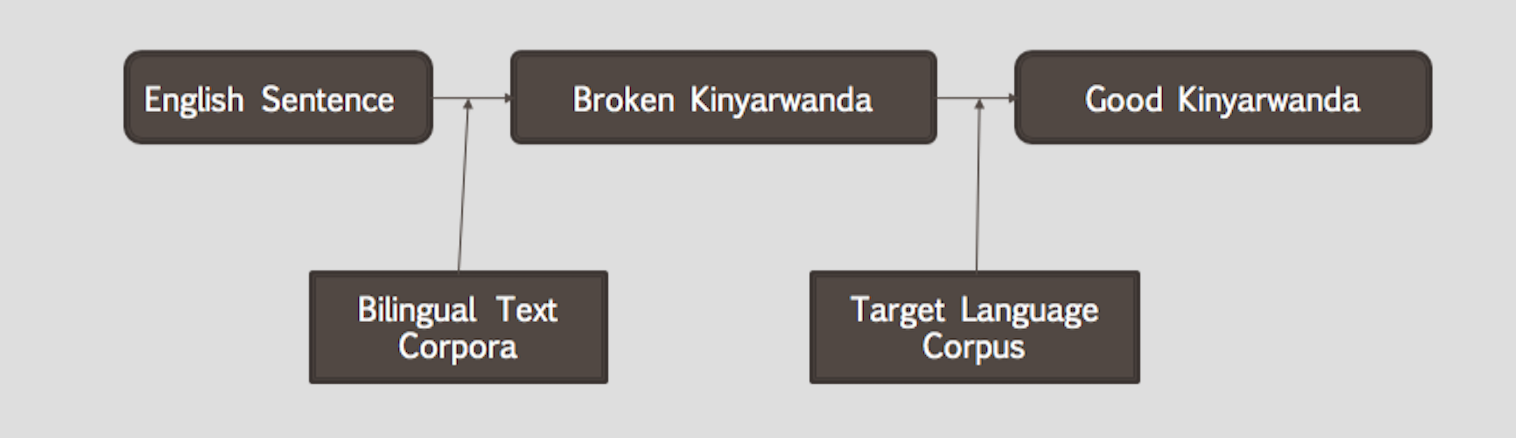
\includegraphics[width=4in]{figures/smt_works.png}
\caption{An illustration of how SMT works. A graphical representation of equation $2.4$.}
\end{center}
\end{figure}

As it can be seen from the above example, Equation $2.4$ is very important. In their article, Brown \textit{et al.} described it as the ``Fundamental Equation of Machine Translation''\cite[p. 265]{brown1993mathematics} as it is capable of summarizing all the three steps involved in translating any given sentence from one language to another by using an SMT-based translation model.

At this point I will focus on the second step of the above-described process as the first and third steps can be easily implemented by a computer program that has access to the date of both the translation model and the target language model, and these two models can be generated by using an SMT system such as Moses in a process that I describe in chapter 3. However before addressing step $2$, let's go back and ask one important question. \textbf{Why is it even necessary to to care about $P(k)*P(e|k)$? Can't we just directly calculate $P(k|e)$ if all we are trying to find is the Kinyarwanda sentence $k_{best}$ that maximize the value of $P(k|e)$?}

Well the answer to that question is rather a devious one. To understand it, we have to look at this question as if we were computer programs. A computer program whose goal is to output the best possible translation $k$ when given an English input sentence $e$ will only care about two things: 
\begin{enumerate}
\item The quality of the output sentence $k$ in the target language (Kinyarwanda in this example).
\item The connection of that output sentence $k$ to the input sentence $e$ that it started with, that is how related are $e$ and $e$ compared to other sentence pairs seen by the translation model in the training and tuning stages.
\end{enumerate}

However, unlike humans, a computer program can't just look at a sentence and decides if it is of good Kinyarwanda quality. It can't also deduce, by just looking at two or more Kinyarwanda sentences, which one is the better translation for a given English sentence. Thus, when in a situation like this, a computer program must reason backwards. At least this is how SMT-based systems are programmed to handle tasks like this one. As long the translation system has access to the translation tables from which it can generate several translations, and assigns to each one of them an exact conditional probability that if we started with that translation, and used the same translation system only going backwards, that is from the target language to the source language, we would get the original English sentence $e$ that we are trying to translate to Kinyarwanda. That conditional probability, combined with the prior probability $p(k)$, enables the translation system to maximize the chance of getting the best possible translation $k$.


For example, the correct Kinyarwanda translation of the English sentence $(e)$: ``\textit{cats and dogs are both mammals}'', is $(k)$: ``\textit{injangwe n' imbwa ni inyamabere zombi}'', with cats = injangwe, and = n', dogs = imbwa, are = ni, both = zombi, mammals = inyamabere. However, we can imagine that our translator, being very smart as it is, may generate the following translation: ``\textit{injangwe n' imbwa ni 
\underline{inyamaswa} zombi}'' $(k')$, which is the translation to ``\textit{cats and dogs are both \underline{animals}}''$(e')$. So even though translation $(k')$ is a good-structured and grammatically-correct Kinyarwanda sentence and would have a high $P(k')$, it is not the correct translation of $(e)$, so its conditional probability, $P(e|k')$, would be low, thus lowering the overall chance that sentence $(k')$ is going to picked as the output by the translator. 

\begin{figure}[h]
\begin{center}
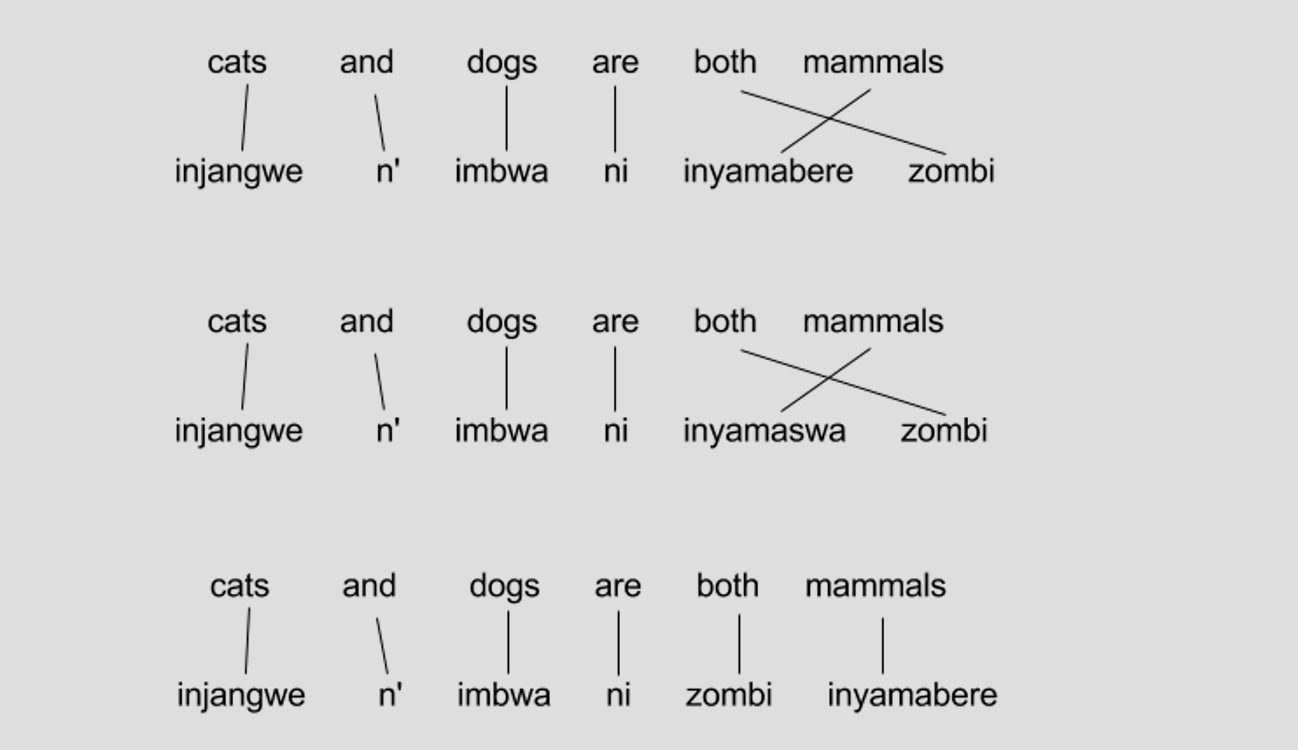
\includegraphics[width=4in]{figures/cats.png}
\caption{Comparison of several possible Kinyarwanda translations of the same English sentence: ``\textit{cats and dogs are both mammals}''.}
\end{center}
\end{figure}
On the other hand, we can imagine a misaligned version of sentence $k$. An example of this case is a sentence like ``\textit{injangwe n'imbwa ni zombi inyamabere}''$(k'')$ which is a one-to-one translation of sentence $(e)$ with each word with the words being in the same posistion as they were previously in $e$. Sentence $k''$ would likely be judged by the translation model as a very good translation. However, if our translation system's Kinyarwanda model was good enough, it would detect the inconsistency in the order of words in $(k'')$ compared to other Kinyarwnda sentences, and $P(k'')$ would be low compared to $P(k)$; however training SMT language models to be very good at detecting minor inconsistencies like this one requires large (more than a billion words) monolingual corpora\cite{och2005statistical}. %An alternative way of addressing this particular common issue of incorrect reordering of words is having a distinct alignments model that is later added to the language model to make sure that cases like the one in the above-mentioned example is correctly dealt with by the translation system. 

Back to our English to Kinyarwanda translation model, we can see that even though the combination of $P(k)$ and $P(e|k)$ is used to make sure that the results of our translation system is as correct as it can get, we can imagine some instances in which the two probabilities may contradict each other, that is when a bigger $P(k)$ means getting a lower $P(e|k)$ or vice versa. In these cases, it is recommended to add weight coefficients to equation $2.3$. Added coefficients depend on the data used in the training and tuning stages, and on the structure of the languages being dealt with.
%%%%%%%%%%%%%%%%%%%%%%%%%%%%%%%%%%%%%%%%%%%%%%%%%%%%%%%%%%%%%%%%%%%%%%%%%%%%%%%%%%%%%%%%%%%%%%%%%%%%%%%%%%%%%%%%%%%%%%%%%%%%%%%%%%%%%%%%%%%%%%%%%%%%%%%%%%%%%%%%%%%%%
\subsection{Alignments}
%%%%%%%%%%%%%%%%%%%%%%%%%%%%%%%%%%%%%%%%%%%%%%%%%%%%%%%%%%%%%%%%%%%%%%%%%%%%%%%%%%%%%%%%%%%%%%%%%%%%%%%%%%%%%%%%%%%%%%%%%%%%%%%%%%%%%%%%%%%%%%%%%%%%%%%%%%%%%%%%%%%%%

As different languages have different structures, and one word from the source language can be translated using zero, one, or multiple words in the target language, it is important that we account for all these possibilities caused by changes in both the structure, and the \textit{fertility} of words in, the language pairs we are working with. The \textit{fertility} of a word is defined as the number of words that are generated by that particular word  when translated from one language to another. To better understand this let's use the following example of a Kinyarwanda - English sentence pair. 
\begin{center}
\begin{tabular}{c}
\begin{lstlisting}
Kinyarwanda: ``Imana yirirwa ahandi igataha i Rwanda.''
English: ``God spends the day elsewhere but spends the night in Rwanda.''
\end{lstlisting}
\end{tabular}
\end{center}

From the above translation, one can immediately deduce that the Kinyarwanda words in the above sentence have higher fertility rates when being translated to English;  however, using this example and doing the translation from English to Kinyarwanda, the English words would have lower fertility rates. 

In the above example, as it can be seen in figure $2.3$, the word ``Imana'' has a fertility of $1$ as it generates one English word, ``God''. On another hand, the word ``yirirwa'' has a fertility of $3$, as it generates a total of three English words (``spends'', ``the'', ``day''). The relationship between Kinyarwanda words and English words illustrated in Figure $2.3$ can also be represented using the Brown \textit{et al.} notation\cite[p. 266]{brown1993mathematics} as following: \textit{(God spends the day elsewhere but spends the night in Rwanda $|$ Imana(1) yirirwa(2, 3, 4) ahandi(5) igataha(7, 8, 9) i(10) Rwanda(11))}. 
In this notation, the numbers in parentheses represent the indexes that the Kinyarwanda words are equivalent to. As you may have noticed, index $6$ is skipped because the English word ``but'' is not connected to any particular word in the Kinyarwanda sentence even.  It is implicitly implied with the structure of the sentence. Such words that are generated somewhat out of nowhere are called ``\textit{spurious}'' words\cite[p. 2]{Germann:2003:GDS:1073445.1073455}.  

However the opposite can also happen. We can imagine translating a Kinyarwanda sentence to English, and losing one of its words through the translation process. In that scenario, that ``\textit{lost}'' word may have been combined with another word and then translated together, or it may have been lost and just been translated through the context of the produced sentence. The ``lost'' word scenario is featured in fig $2.4$.

\begin{figure}[h]
\begin{center}
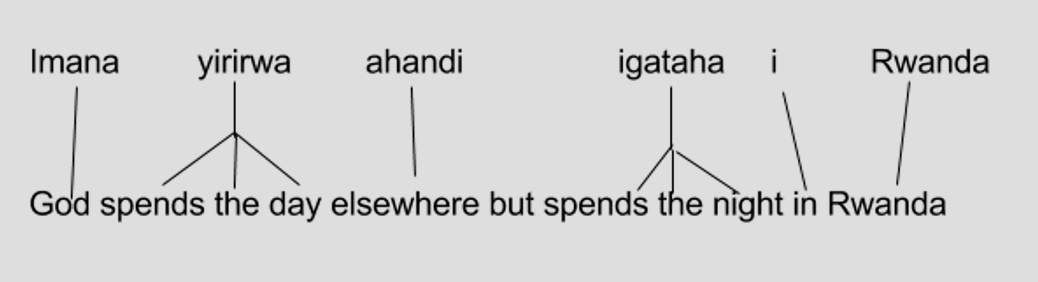
\includegraphics[width=4in]{figures/fig-one.png}
\caption{An example of sentence alignment with a ``spurious'' word: ``\textit{but}''.}
\end{center}
\end{figure}
\begin{figure}[h]
\begin{center}
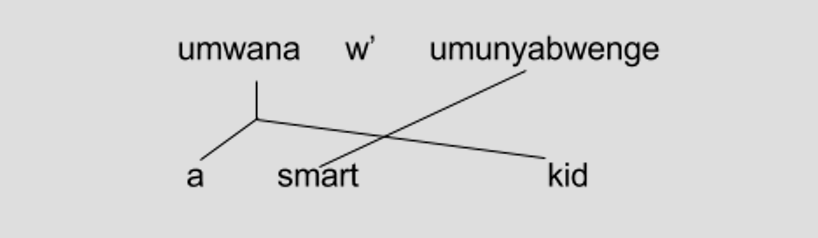
\includegraphics[width=4in]{figures/fig-two.png}
\caption{Example of a sentence alignment with a ``lost'' word: ``\textit{w'}''.}
\end{center}
\end{figure}
\begin{figure}[h]
\begin{center}
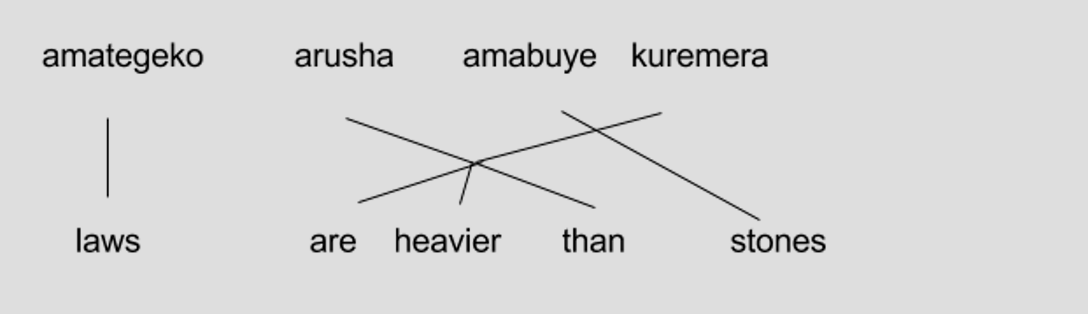
\includegraphics[width=4in]{figures/fig-three.png}
\caption{A sentence pair alignment containing both ``lost'' and ``spurious'' words.}
\end{center}
\end{figure}

However most sentence pairs that are dealt with during the training stage or the translation process do not just contain spurious words or lost words but a mixture of both (e.g.: Figure $2.5$); and that is why alignment probabilities should be assigned to these two possibilities when developing a translation model.  Depending on which language pair you are dealing with, ``lost'' and ``spurious'' words can have a very significant impact on the quality of the translation results. They ought to be taken seriously. 

According to Brown \etal\cite[p. 268]{brown1993mathematics}, the way that SMT decoders use to handle these irregular cases of alignments is by adding one empty \textit{cept}\footnote{In this case, \textit{cept} is defined as a word or a group of words whose context is translated together.} to the sentence about to be translated, and using it as an alignment partner for any ``spurious'' word found in the final translation. As for ``lost'' words, Brown \textit{at al.}\cite[p. 268]{brown1993mathematics} suggest using their implied meaning or context to align them with their closest or related counterparts in the target language sentence.


By applying these suggestions to the example illustrated in Figure $2.4$, we would get the following alternative alignment: \textit{(a smart kid $|$ $k_0$(1)  umwana(1) w'(2) umunyabwenge(2))}, where $k_0$, stand for the null cept that we placed at the beginning of the Kinyarwanda string before translating it to English. Also notice how instead of skipping the string \textit{``w'''}, we now combine it with the string \textit{``umunyabwenge''} into a context-based cept \textit{``w' umunyabwenge''}, and then translate both words together together to the English cept, \textit{``smart''}. In this case, the cept is just one word, but we can imagine cases in which it is empty or contains multiple words.

One important question that arises as these two suggestions are implemented together is that there are many alignments for each translation pair. If you showed the alignments in Figures $2.4$ and $2.5$ to a group of ten people, it is unlikely that they all would agree that one alignment is better than the other one. Based on this, one can imagine what an SMT-based translation model is going when presented with not one, but $2^{lm}$ possible alignments for each sentence pair with $l$ being the number of words in the source language sentence, and $m$, the number of words in its target language sentence. 
\begin{figure}[h]
\begin{center}
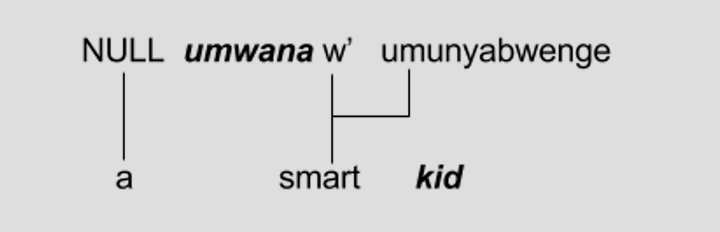
\includegraphics[width=4in]{figures/fig-four.png}
\caption{An alignment in which \textit{``w' umunyabwenge''} is aligned with ``\textit{smart}''}
\end{center}
\end{figure}
\begin{figure}[h]
\begin{center}
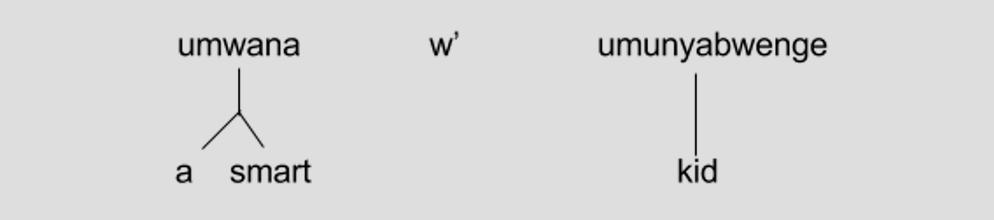
\includegraphics[width=4in]{figures/fig-five.png}
\caption{A graphical representation of another less likely (incorrect) alignment of the sentence pair: ``\textit{a smart kid $|$  umwana w' umunyabwenge}''.}
\end{center}
\end{figure}

To handle this challenge of having several possible alignments for every sentence pair, according to Brown \textit{at al.}\cite[p. 269-270]{brown1993mathematics}, an SMT model has to assign a likelihood probability to each possible alignment. For example, for the \textit{(a smart kid $|$ umwana w' umunyabwenge)} translation pair, both the alignments in Figures $2.4$ and $2.5$ would have bigger probabilities while alignments such as \textit{(a smart kid $|$ umwana(1, 2, 3) w' umunyabwenge)} and \textit{(a smart kid $|$ umwana(1) w'(2) umunyabwenge(3))} would have lower probabilities as they are incorrect, thus less likely to be considered by the translation model.

\section{Phrase-Based Translation Model}
Several SMT systems now use a phrase-based translation model to build phrase translation tables that are more effective than tables generated by word-based alignments \cite[p. 48]{koehn2003statistical}. The reason why phrase-based models outperform word-based models is because phrase-based models break each sentence into phrase segments that are then translated and reconstructed later into the target language. This gives phrase-based translation systems the ability to account for contexts and meanings that words have used alongside some other particular words as opposed to when used alone or with different words. This is taking advantage of statistical probabilities that were in generated from the parallel corpora data used during the training and tuning stages. 

An obvious case in which a phrase-based model would perform better than a word-based model is in the translation of sentences that contain idiomatic expressions. As an example, translating an expression like \textit{cutting corners}\footnote{To cut corners is ``to do something in the easiest, cheapest, or fastest way''\cite{cutcornerscambridge}.} using a word-based translation system would result in the loss of contextual meaning that the words \textit{cutting} and \textit{corners} have when used together in the expression \textit{cutting corners}.

